\documentclass{beamer}

% german content
\usepackage[ngerman]{babel}

% bibliography
\usepackage[
  backend=biber,
  style=authoryear,
  citestyle=authoryear,
  autocite=footnote
]{biblatex}
\addbibresource{bibliography.bib}

% images
\usepackage{graphicx}
\graphicspath{ {./images/} }

\usepackage[normalem]{ulem}

\title{Peer-to-Peer Volltextsuche}
\subtitle{}
\author{
  Boris Caspary \\
  Emma Calewaert \\
  Jonathan Neidel \\
  Joscha Seelig \\
  Leon Enzenberger \\
  Ryan Torzynski \\
  Simon Breiter \\
  Stefan Sadewasser \\
}
\date{Juli 2021}
\institute{HTW Berlin, Angewandte Informatik, Projektstudium bei Herr Hoppe}
\logo{
\includegraphics[width=1cm]{logo}}

% theme + color theme
\usetheme{Szeged}
\usecolortheme{whale}
% see: https://deic-web.uab.cat/~iblanes/beamer_gallery/index.html
\setbeamerfont{caption}{size=\Tiny}

\begin{document}
\frame{\titlepage}

\section{Projektidee}
\begin{frame}
  \begin{center}
    {\Huge Projektidee}
  \end{center}
\end{frame}

\begin{frame}[allowframebreaks]
  \frametitle{Basiskonzepte}
  Peer-to-peer
  \begin{itemize}
    \item Rechnernetz
    \item Gleichtberechtigte Knoten
  \end{itemize}

  \break
  Volltextsuche
    \begin{itemize}
    \item Finden von Wörtern
    \item Handelt sich um Texte
    \item Zwei Phasen: Indexierung- und Anfragephase
  \end{itemize}
\end{frame}

\begin{frame}
  \frametitle{Bundestagsreden}
  \begin{columns}
    \begin{column}{0.5\textwidth}
      \begin{itemize}
        \item Protokolle als Open Data verfügbar
        \item Großer Umfang an Daten (+/- 33 000 Reden)
        \item XML-Dateien*
      \end{itemize}
    \end{column}
    \begin{column}{0.5\textwidth}
      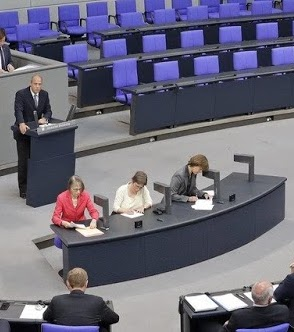
\includegraphics[width=5cm]{BundestagProtokoll}
      {\tiny Bildquelle: Deutscher Bundestag / Thomas Köhler/ photothek.net}
    \end{column}
  \end{columns}
\end{frame}

\begin{frame}[allowframebreaks]
    \hspace*{-10.75mm}
    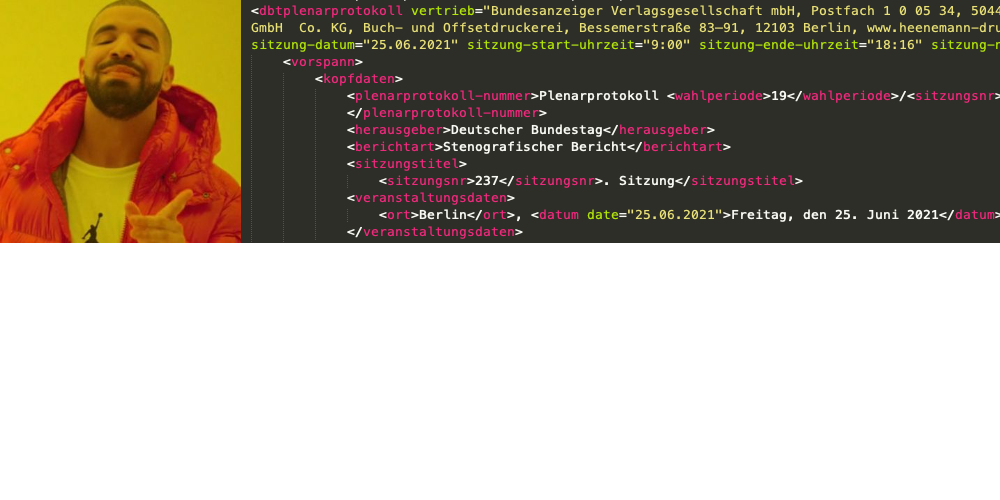
\includegraphics[width=\paperwidth]{drakememe-only-19}

    \break

    \hspace*{-10.75mm}
    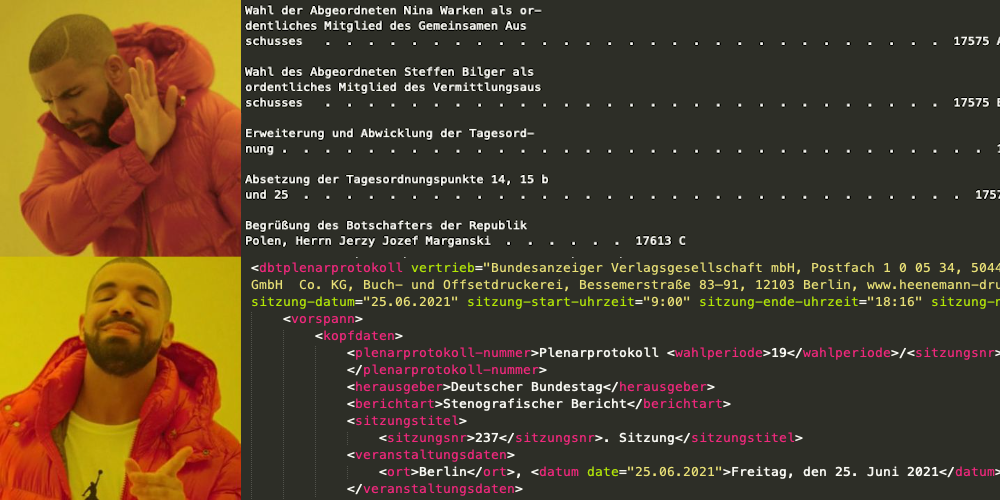
\includegraphics[width=\paperwidth]{drakememe}
\end{frame}

\section{Aufgabenteilung}
\begin{frame}
  \begin{center}
    {\Huge Aufgabenteilung}
  \end{center}
\end{frame}

% \begin{frame}[allowframebreaks]
%   \frametitle{Arbeitspakete}

%   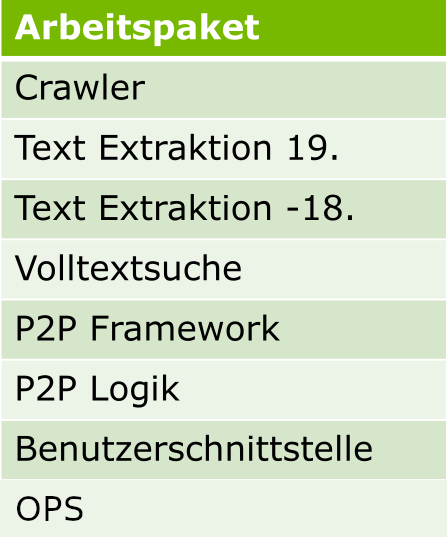
\includegraphics[width=5cm]{Arbeitspakete}
%   \break
%   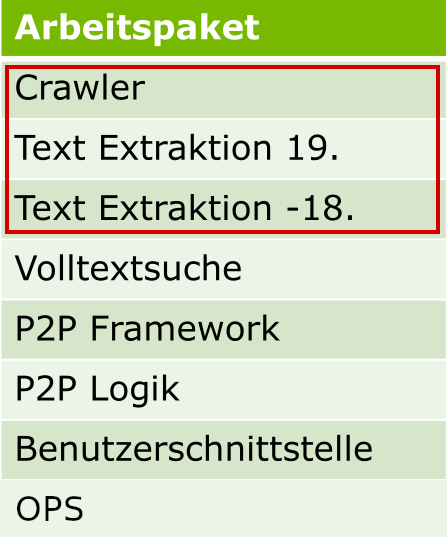
\includegraphics[width=5cm]{Arbeitspakete-Crawler}
%   \break
%   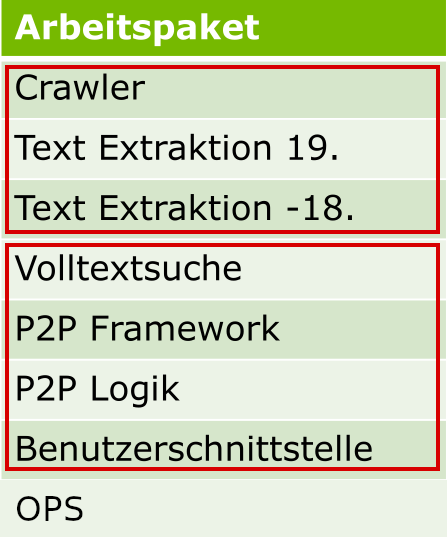
\includegraphics[width=5cm]{Arbeitspakete-Main}
% \end{frame}

\begin{frame}
  \frametitle{Schichtenmodell}

  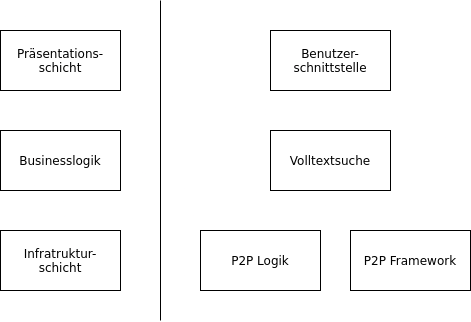
\includegraphics[width=8cm]{Schichten}
\end{frame}

\section{Peer-to-Peer}
\begin{frame}
  \frametitle{Peer-to-Peer}
  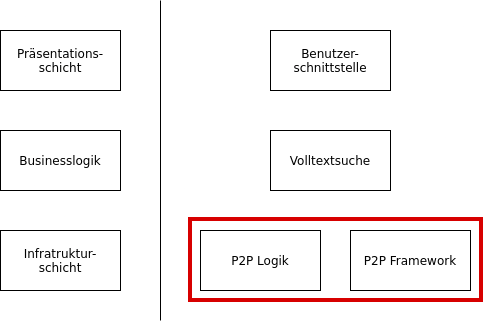
\includegraphics[width=8cm]{Schichten-p2p}
\end{frame}

\begin{frame}
  \frametitle{DHT}

  \begin{itemize}
    \item Distributed
    \item Hash Table
  \end{itemize}
\end{frame}

\begin{frame}
  \frametitle{Hash Table}

  \begin{itemize}
    \item key-value store
  \end{itemize}

  \medskip

  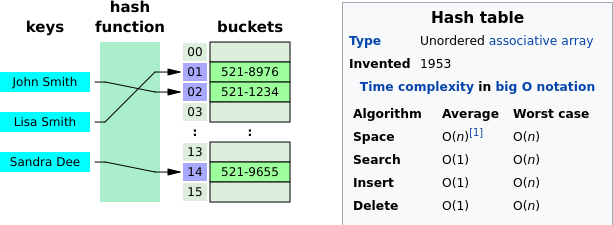
\includegraphics[width=8cm]{ht}

  \medskip

  {\tiny Bildquelle: https://en.wikipedia.org/wiki/Hash\_table}
\end{frame}

\begin{frame}[allowframebreaks]
  \frametitle{Distributed HT}

  
\includegraphics[width=8cm]{dht1}

  \break

  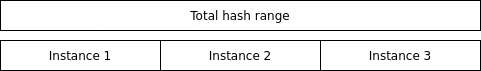
\includegraphics[width=8cm]{dht2}

  \break

  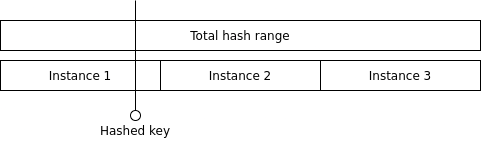
\includegraphics[width=8cm]{dht3}
\end{frame}

\begin{frame}
  \frametitle{Schichten}

  \begin{center}
    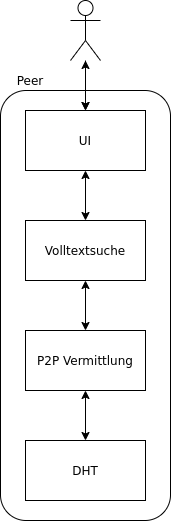
\includegraphics[height=6cm]{Schichten-alt}
  \end{center}
\end{frame}

\begin{frame}
  \frametitle{Verteilung des Systems}

  Design Entscheidung:

  Wie soll die Funktionalität des Systems verteilt werden?
\end{frame}

\begin{frame}[allowframebreaks]
  \frametitle{1. Zentralisierung}

  \begin{center}
    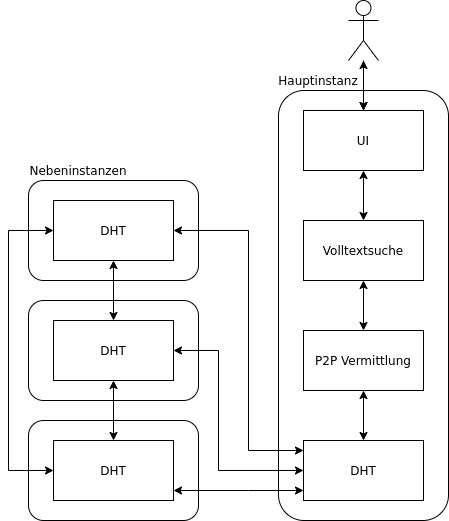
\includegraphics[height=6cm]{Hauptinstanz}
  \end{center}

  \break
  Pro:
  \begin{itemize}
    \item zentrale Anlaufstelle (Nutzerfreundlich)
  \end{itemize}

  Con:
  \begin{itemize}
    \item zentrale Anlaufstelle (single point of failure)
    \item Load nicht verteilt
  \end{itemize}
\end{frame}

\begin{frame}[allowframebreaks]
  \frametitle{2. Pur}

  \begin{center}
    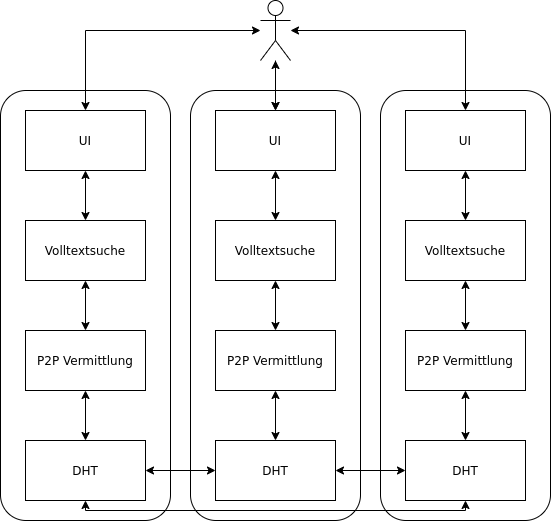
\includegraphics[height=6cm]{Gleichberechtigt}
  \end{center}

  \break
  Pro:
  \begin{itemize}
    \item Load verteilt
    \item mehrere Anlaufstellen (kein single point of failure)
  \end{itemize}

  Con:
  \begin{itemize}
    \item mehrere Anlaufstellen (verwirrte Nutzer $\rightarrow$ Loadbalancer)
    \item Administrationsaufwand ($\rightarrow$ OPS)
  \end{itemize}

  \bigskip

  Unsere Wahl
\end{frame}

\section{Volltextsuche}
\begin{frame}
  \frametitle{Volltextsuche}

  \begin{center}
    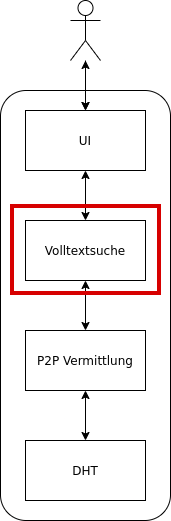
\includegraphics[height=6cm]{Schichten-alt-volltext}
  \end{center}
\end{frame}

\begin{frame}
  \frametitle{Volltextsuche}

  Modi:
  \begin{enumerate}
    \item Indexierungsphase
      \begin{enumerate}[a]
        \item Aufbereitung der Daten
        \item Einfügen in Invertierten Index
      \end{enumerate}
    \item Anfragephase
  \end{enumerate}
\end{frame}

\begin{frame}[allowframebreaks]
  \frametitle{1a. Aufbereiten der Daten}

  Beispiel:

  Klaus-Rüdiger steht vor dem Hause der CDU.

  \break

  \textbf{Tokenisierung:}

  \begin{itemize}
    \item Segmentierung in einzelne Wörter
    \item Lowercase
    \item Satzzeichen entfernen
  \end{itemize}

  \bigskip
  'klaus-rüdiger' 'steht' 'vor' 'dem' 'hause' 'der' 'cdu'

  \break

  \textbf{Stopwörter entfernen:}

  \medskip

  {\scriptsize
    \begin{itemize}
      \item Pronomen (ich, ihre, ..)
      \item Konjunktionen (und, aber, ..)
      \item Präposition (auf, bis, ..)
      \item Artikel (der, die, ..)
    \end{itemize}
  }

  \bigskip

  'klaus-rüdiger' 'steht' \sout{'vor'} \sout{'dem'} 'hause' \sout{'der'} 'cdu'

  \break

  \textbf{Stemming:}

  \bigskip

  \begin{itemize}
    \item Zurückführung auf den Wortstamm
    \item Snowball Stemming
  \end{itemize}

  \bigskip

  \textbf{'klaus-rüdiger' $\rightarrow$ 'klaus-rudig'} 'steht' \textbf{'hause' $\rightarrow$ 'haus'} 'cdu'

  \break

  \textbf{Normalisierung:}

  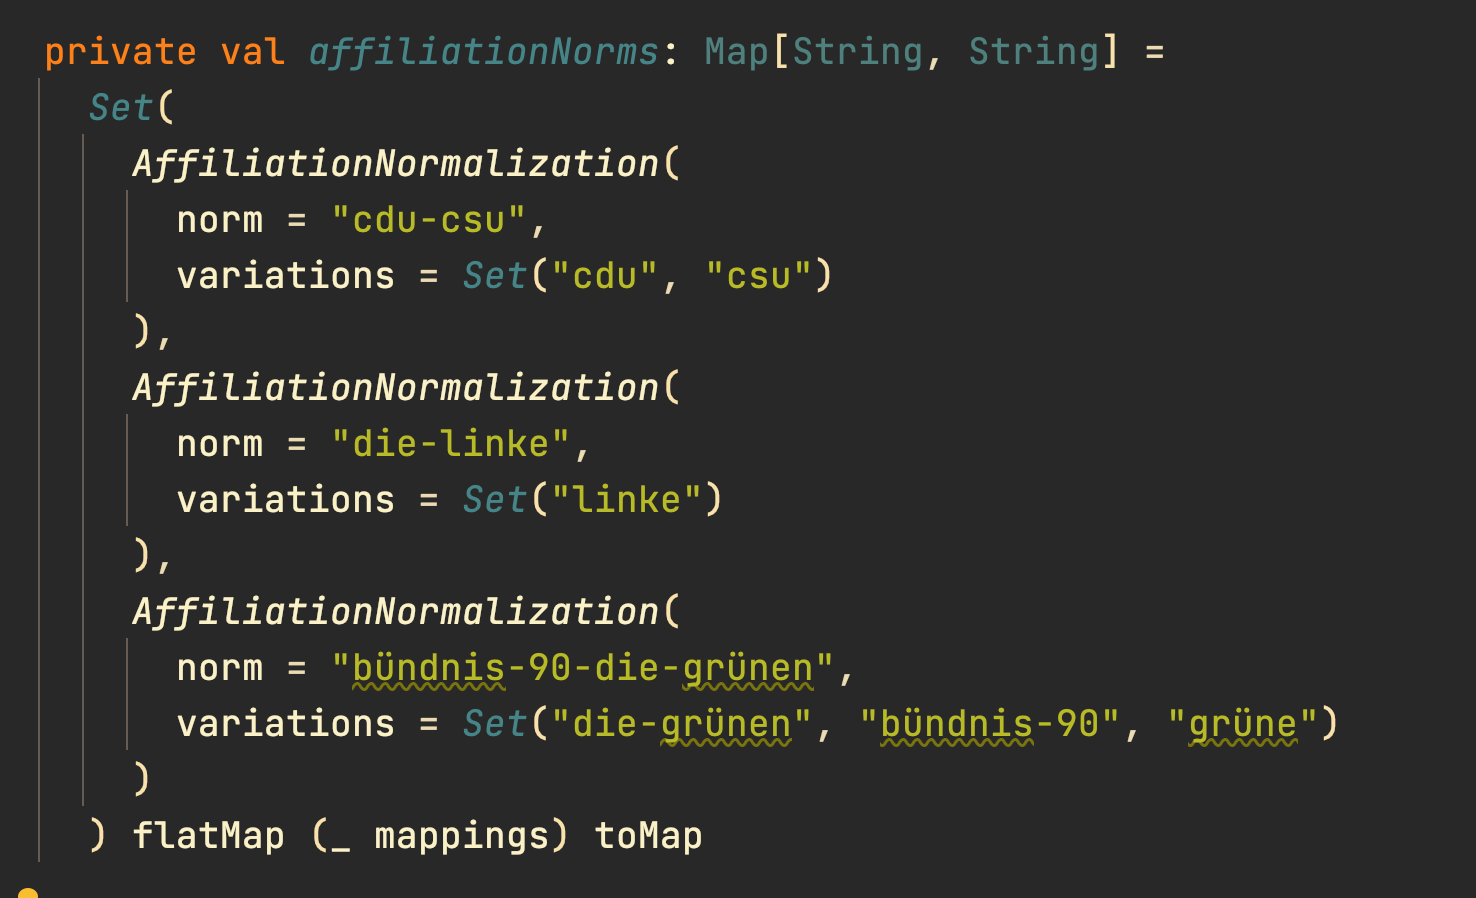
\includegraphics[width=8cm]{normalisierung}

  \bigskip

  'klaus-rudig' 'steh' 'haus' \textbf{'cdu' $\rightarrow$ 'cdu-csu'}
\end{frame}

\begin{frame}
  \frametitle{1b. Inverted Index}

  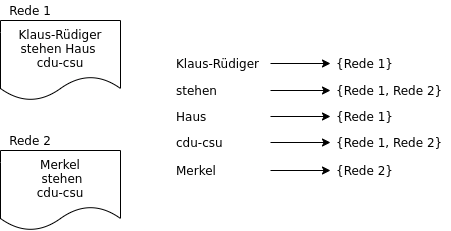
\includegraphics[width=8cm]{inverted-index}
\end{frame}

\begin{frame}
  \frametitle{1b. Distributed Inverted Index}

  Einfügen in den DHT

  \medskip

  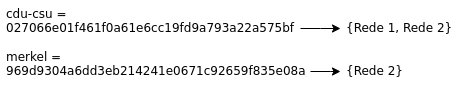
\includegraphics[width=8cm]{distributed-inverted-index}
\end{frame}

\begin{frame}[allowframebreaks]
  \frametitle{1b. Aufteilung der Daten}

  Design Entscheidung:

  Wie sollen die Daten aufgeteilt werden?

  \break

  % \textbf{1. Nach Partei}

  % Pro Partei ein Peer zuständig

  % Pro:
  % \begin{itemize}
  %   \item Schnell beim Einfügen
  %   \item Schnell beim Abrufen wenn nach Partei gefiltert
  % \end{itemize}
  % Con:
  % \begin{itemize}
  %   \item Sonst langsam
  %   \item Load Imbalance
  %   \item Benachteiligung einer Partei wenn Peer down
  % \end{itemize}

  % \break

  \textbf{1. Partition by Keyword}

  \begin{itemize}
    \item Gleichmäßige Verteilung der Keywords über DHT
    \item Speicherung in Distributed Inverted Index
  \end{itemize}

  \bigskip

  Pro:
  \begin{itemize}
    \item Schnell beim Abrufen von Keywords
  \end{itemize}

  Con:
  \begin{itemize}
    \item Langsam beim Einfügen
      \begin{itemize}
        \item $\rightarrow$ Relevanz für den Use Case
        \item $\rightarrow$ bei uns: 2-3 min pro Protokoll
        \item Optimierungen möglich
      \end{itemize}
  \end{itemize}

  \break

  \textbf{2. Partition by Document}

  \begin{itemize}
    \item Gleichmäßige Verteilung der Dokumente über Peers
    \item Speicherung in lokalem Invertiertem Index
  \end{itemize}

  \bigskip

  Pro:
  \begin{itemize}
    \item Schnell beim Einfügen (lokales Speichern in Sekunden)
  \end{itemize}
  Con:
  \begin{itemize}
    \item Abruf langsam (Fluten des Netzwerks)
    \item Schlechte Skalierbarkeit
  \end{itemize}
\end{frame}

\begin{frame}
  \frametitle{2. Anfragephase}

  \begin{itemize}
    \item Aufbereiten der Suchbegriffe (Tokenisierung, etc.)
    \item Abrufen der Daten aus Distributed Inverted Index
    \item Bewertung der Relevanz (sortieren)
  \end{itemize}
\end{frame}

\section{Demo}
\begin{frame}
  \frametitle{UI Demo}

  \begin{center}
    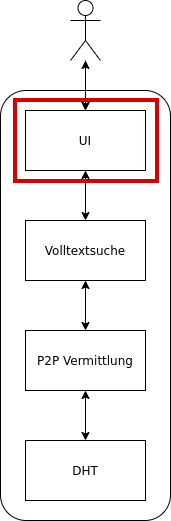
\includegraphics[height=6cm]{Schichten-alt-ui}
  \end{center}
\end{frame}

\end{document}
